\chapter{Programowanie mikrokontrolerów ARM}
Procesory ARM posiadają architekturę 32 lub 64 bitową. Z uwagi na energooszczędną konstrukcję używane są przede wszystkim w systemach wbudowanych, w nich niski pobór energii jest jedną z ważniejszych kwestii. Obecnie stały się bardzo popularne i używane są już w niemal każdym urządzeniu mobilnym, np. telefon komórkowy, dyski twarde itp.

Poniższy rozdział prezentuje w jaki sposób należy kompilować program, aby był wykonalny przez procesor o architekturze ARM oraz jak najwygodniej skonstruować środowisko programistyczne, aby praca z kodem była jak najłatwiejsza.

\section{Środowisko programowania}
Kod programu oraz obsługi stacji pogody, zaimplementowanej na mikrokontrolerze BeagleBone Black, został napisany przy użyciu środowiska programistycznego Eclipse. Środowisko to zostało wybrane przez wzgląd na ogromne możliwości, które ułatwiają w znacznej mierze programowanie oraz skracają jego czas. Eclipse jest darmowym narzędziem do programowania, jest intuicyjny w obsłudze, a przede wszystkim posiada wielką rzeszę użytkowników, przez co w przypadku problemów, ich rozwiązanie jest niemal natychmiastowe. Środowisko to można pobrać z oficjalnej strony, w projekcie został wykorzystany \emph{Eclipse IDE for C/C++ Developers}.

\begin{figure}[h]
\centering
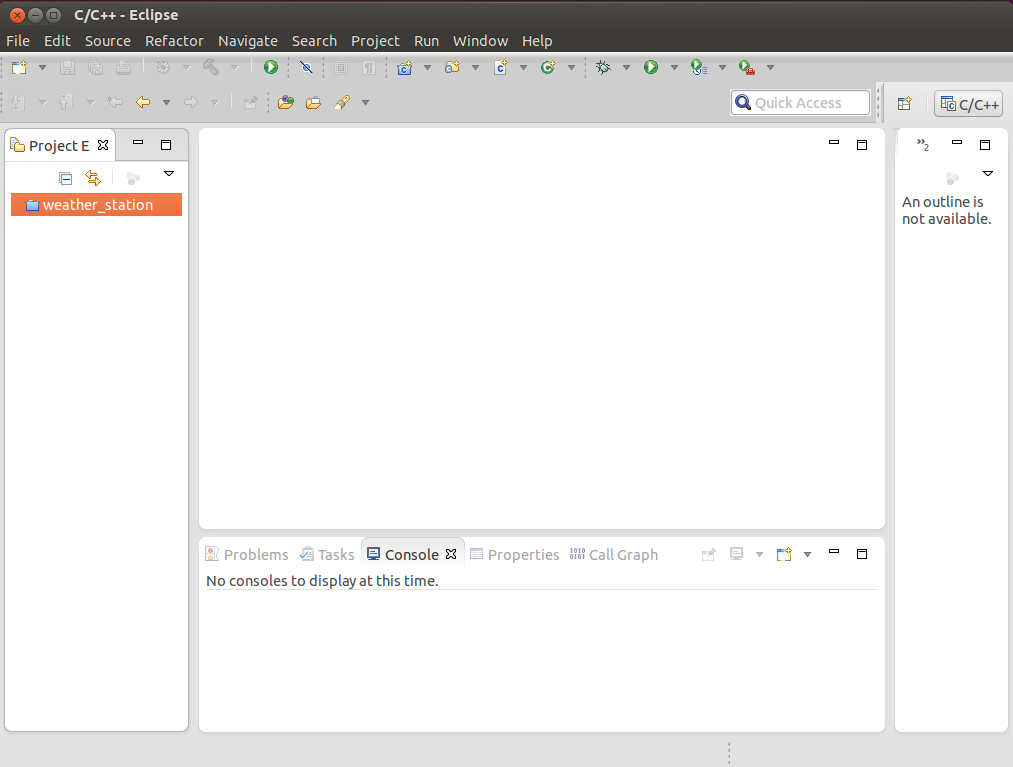
\includegraphics[scale=0.36]{eclipse}
\caption{Główny wygląd Eclipse'a}
\label{fig:eclipse}
\end{figure}

Po rozpakowaniu gotowego środowiska oraz jego uruchomieniu można już zacząć pracę z mikrokontrolerem, wystarczy jeszcze dokonać parę zabiegów, aby czas od zbudowania projektu, do jego uruchomienia na BeagleBone'ie był jak najkrótszy. W celu uzyskania jak najwygodniejszej konfiguracji, Eclipse został uruchomiony na systemie operacyjnym Ubuntu, na którym były przechowywane wszystkie źródła. Dzięki odpowiedniemu dodatkowi do Eclipse'a - Remote System Explorer istnieje możliwość tworzenia programu na komputerze, jego cross-kompilacji do aplikacji wykonywalnej oraz uruchomienia gotowego pliku binarnego na mikrokontrolerze. Dzieje się to dzięki wspomnianemu wcześniej protokołowi SSH.

Aby stworzyć nowy projekt należy kliknąć File->New->C Project (może być również C++), pojawi się okno pokazane na rysunku \ref{fig:eclipse_new}:

\begin{figure}[h!]
\centering
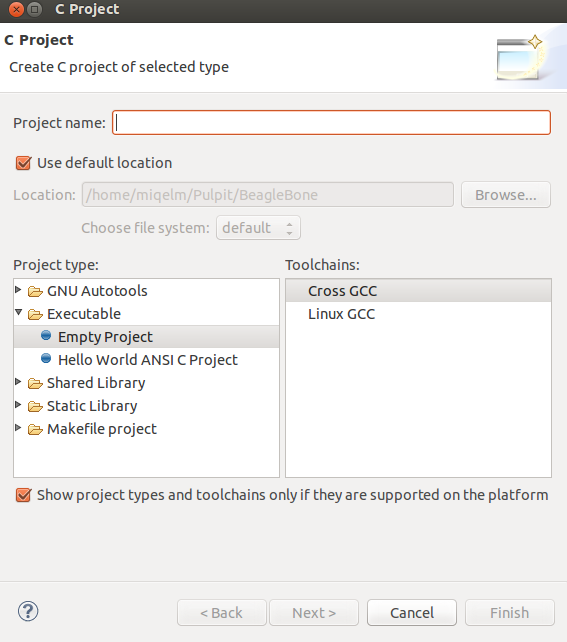
\includegraphics[scale=0.36]{eclipse_new}
\caption{Tworzenie nowego projektu}
\label{fig:eclipse_new}
\end{figure}

Po uzupełnieniu nazwy projektu oraz wyboru Cross GCC, należy przejść dalej i zakończyć konfigurację. Teraz następuje najważniejsza rzecz. Aby skompilować projekt i móc go uruchomić na innej platformie sprzętowej, jaką jest procesor ARM, potrzebny jest cross-kompilator. Jest to wymagane, gdyż komputer oraz BeagleBone różnią się budową oraz sposobem komunikacji na najniższym poziomie. W związku z tym, należy na komputerze zainstalować narzędzie umożliwiające generowanie pliku binarnego na inną platformę sprzętową, proces ten jest nazywany cross-kompilacją.

BeagleBone Black jest wyposażony w procesor o architekturze ARM hard float, dlatego też potrzebny jest do niego kompilatora, nazywa się on \emph{arm-linux-gnueabihf-gcc}. Aby go zainstalować, należy w konsoli użytkownika wpisać następującą komendę:\newline
\emph{sudo apt-get install arm-linux-gnueabihf-gcc}\newline
Potwierdzając chęć zainstalowania oraz pomyślnym przebiegu instalacji, można teraz skompilować program na architekturę ARM.

W Eclipse klikając teraz prawym przyciskiem myszy na nowo stworzony projekcie, następnie wciśnięciu Properties, ukazują się właściwości projektu. Należy teraz zakomunikować środowisku, że program będzie kompilowany przy użyciu zainstalowanego przed chwilą kompilatora. W tym celu należy uruchomić zakładkę C/C++ Build, a potem opcję Settings i Cross GCC Compiler, w polu Command należy wpisać nazwę cross-kompilatora. Poniżej zostaje zamieszczony zrzut ekranu przedstawiający zaistniałą sytuację:

\begin{figure}[h]
\centering
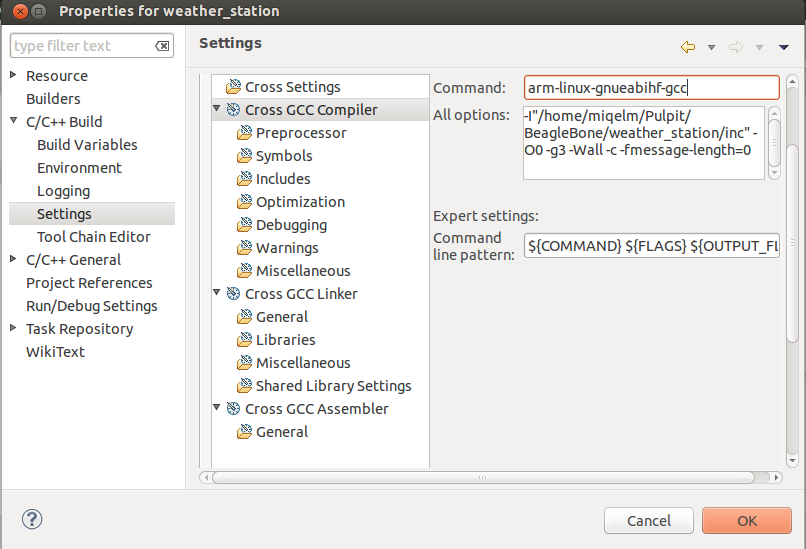
\includegraphics[scale=0.36]{eclipse-settings}
\caption{Ustawienia projektu}
\label{fig:eclipse-settings}
\end{figure}

W podobny sposób należy wypełnić również pola Command w zakładkach Cross GCC Linker oraz Cross GCC Assembler, ten ostatni należy wypełnić wpisując: arm-linux-gnueabihf-as.

Tak przygotowany projekt wraz z zainstalowanym cross-kompilatorem umożliwia użytkownikowi bezproblemowe skompilowanie całego projektu do jednego pliku wykonywalnego. Otrzymany plik binarny należy przy użyciu protokołu SSH przesłać do BeagleBone'a i tam go uruchomić.

\section{Używanie bibliotek Linux'a}
System Linux w swoim jądrze posiada zaimplementowaną ogromną ilość przydatnych funkcji. Przy tworzeniu systemu pomiarów warunków meteorologicznych użyta została biblioteka funkcji do obsługi magistrali  $\mathrm{I^{2}C}$.

Funkcje te znacznie ułatwiły odczyt i zapis do czujnika BMP085, który działa tylko i wyłącznie w wymienionym poniżej sposobie komunikacji. Lista funkcji użytych w tworzeniu projektu:

\begin{itemize}
\setlength{\itemsep}{2pt} 
\setlength{\parskip}{2pt} 
\setlength{\parsep}{2pt}
\item i2c\_smbus\_read\_word\_data - sluzy do odczytywania 16 bitów spod adresu podanego w argumencie
\item i2c\_smbus\_write\_byte\_data - zapis podanego bajtu pod odpowiedni adres w pamięci urządzenia w magistrali
\item i2c\_smbus\_read\_byte\_data - odczyt bajtu z odpowiedniego adresu urządzenia
\end{itemize}